\kommentar{Wellen \& Strahlungsfelder}  %Thema

\begin{karte}{Was beschreibt das Poynting-Theorem?}
	Grundsätzlich handelt sich beim Poynting-Theorem um Energieerhaltung mit Leistungsübertragung.
	
	\begin{equation*}
	\underbrace{-\frac{d}{d t} \int_{V}\left(w_{e}+w_{m}\right) d v}_{\text{ Zeitliche Änderung der Energie }}
	=
	\underbrace{\int_{V} p d v}_{\text{Leistung}}
	+
	\underbrace{\int_{A=\partial V} \vec{S} \cdot d \vec{s}}_{Leistungsübertragung}
	\end{equation*}
	
	Die Zeitliche Änderung der Energie in einem Volumen, sei sie nun zugeführt oder abgeführt worden, muss gleich gross sein wie die Abgegebene Leistung (Wärme, bei zugeführte Leistung bspw. Solarzelle) plus der austretende oder eintretende Leistung des Volumens.
\end{karte}

\begin{karte}{Was bezeichnet der Poynting Vektor?}
	\begin{equation*}
	\vec{S}=\vec{E} \times \vec{H}
	\end{equation*}
	
	Der Poynting Vektor ist die Leistungsdichte einer Fläche und hat somit die Einheit $[S] = \dfrac{W}{m^2}$.\\
	Der Vektor zeig in die Richtung der Leistung.\\[5pt]
\end{karte}

\begin{karte}{Was besagt die spezielle Relativitätstheorie für die Elektrodynamik?}
	\textbf{Das elektrische und das magnetische Feld sind verschiedene Wirkungsweisen von demselben Phänomen}\\
	Alles kommt auf das Bezugssystem an. Wenn wir uns mit dem Strom mit bewegen sehen wir nur die elektrische Wirkung. Wenn wir uns nicht bewegen, sehen wir die magnetische Wirkung des Stroms.\\
	Wenn wir uns bewegen verhält sich die Zeit anders. Dies wirkt sich bspw. bei der Verkürzung von Längen aus.\\
	Es gibt auch Effekte welche nicht durch die Bewegung beeinflusst werden. z.B. ist die Ladung immer gleich.
\end{karte}

\begin{karte}{Was bedeutet die Polarisation von elektromagnetischen Wellen?}
	Die Polarisation ist die Richtung des Elektrischen Felds.\\
	Die Welle ist x-Polarisiert wenn der E-Feld Vektor in x Richtung zeigt.\\
	%Autor: Simon Walker
%Version: 1.0
%Datum: 29.11.2019
%Lizenz: CC BY-NC-SA

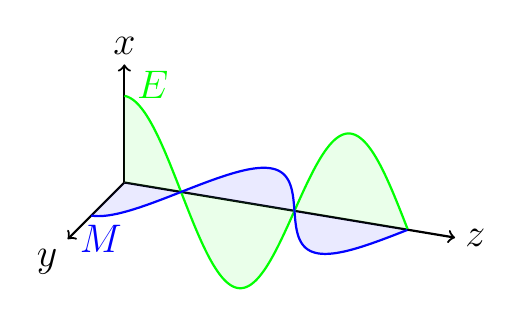
\begin{tikzpicture}[x={(0,1cm)}, y={(-0.6cm,-0.6cm)}, z={(1.2cm, -0.2cm)}]
		
	\def\cycles{1.25} %Anz Schwingungen
	\def\lenght{3}%länge in z richtung
	
	
	\draw [->, thick] (0,0,0)  -- (1.5,0,0) node[above] {\Large$x$};
	\draw [->, thick] (0,0,0) -- (0,1.2,0) node[below left] {\Large$y$};
	\draw [->, thick] (0,0,0) -- (0,0,\lenght+0.5) node[right] {\Large$z$};
	
	\draw[thick, green] %E-Feld Plot
	plot[domain=0:\lenght, samples=200] 
	({1.1*cos(deg(2*\cycles*pi*\x/\lenght))}, 0, \x);
	
	\draw[thick, blue] %M-Feld Plot
	plot[domain=0:\lenght, samples=200] 
	(0, {0.7*cos(deg(2*\cycles*pi*\x/\lenght))}, \x);
	
	\fill[opacity=.1,green!80] %E-Feld füllung
	(0,0,0) --
	plot[domain=0:\lenght, samples=200] 
	({1.1*cos(deg(2*\cycles*pi*\x/\lenght))}, 0, \x)  --
	(0,0,0);
	
	\fill[opacity=.1,blue!80] %M-Feld füllung
	(0,0,0) --
	plot[domain=0:\lenght, samples=200] 
	(0, {0.7*cos(deg(2*\cycles*pi*\x/\lenght))}, \x)  --
	(0,0,0);
	
	\node[green] at (1.3,0,0.3) {\Large$E$}; %Beschriftungen
	\node[blue] at (0,1.1,0.3) {\Large$M$};
	
\end{tikzpicture}

\end{karte}

\begin{karte}{Was ist die Ausbreitungsgeschwindigkeit von elektromagnetischen Wellen?}
	\Large
	\begin{equation*}
		v_{ph} = \frac{1}{\sqrt{\varepsilon \cdot \mu}}
	\end{equation*}	
	 \normalsize
	Somit ist die Ausbreitungsgeschwindigkeit im Vakuum:
	\begin{equation*}
		v_{ph_{Vakuum}} = \frac{1}{\sqrt{\varepsilon_0 \cdot \mu_0}} = c
	\end{equation*}
	
\end{karte}

\begin{karte}{Was versteht man unter einer ebenen Welle?}
	Das magnetische Feld und das elektrische Feld stehen senkrecht zueinander und die Welle ist Harmonisch.\\
\end{karte}
